\documentclass{standalone}
\usepackage{tikz}
\usetikzlibrary{patterns, positioning}

\begin{document}
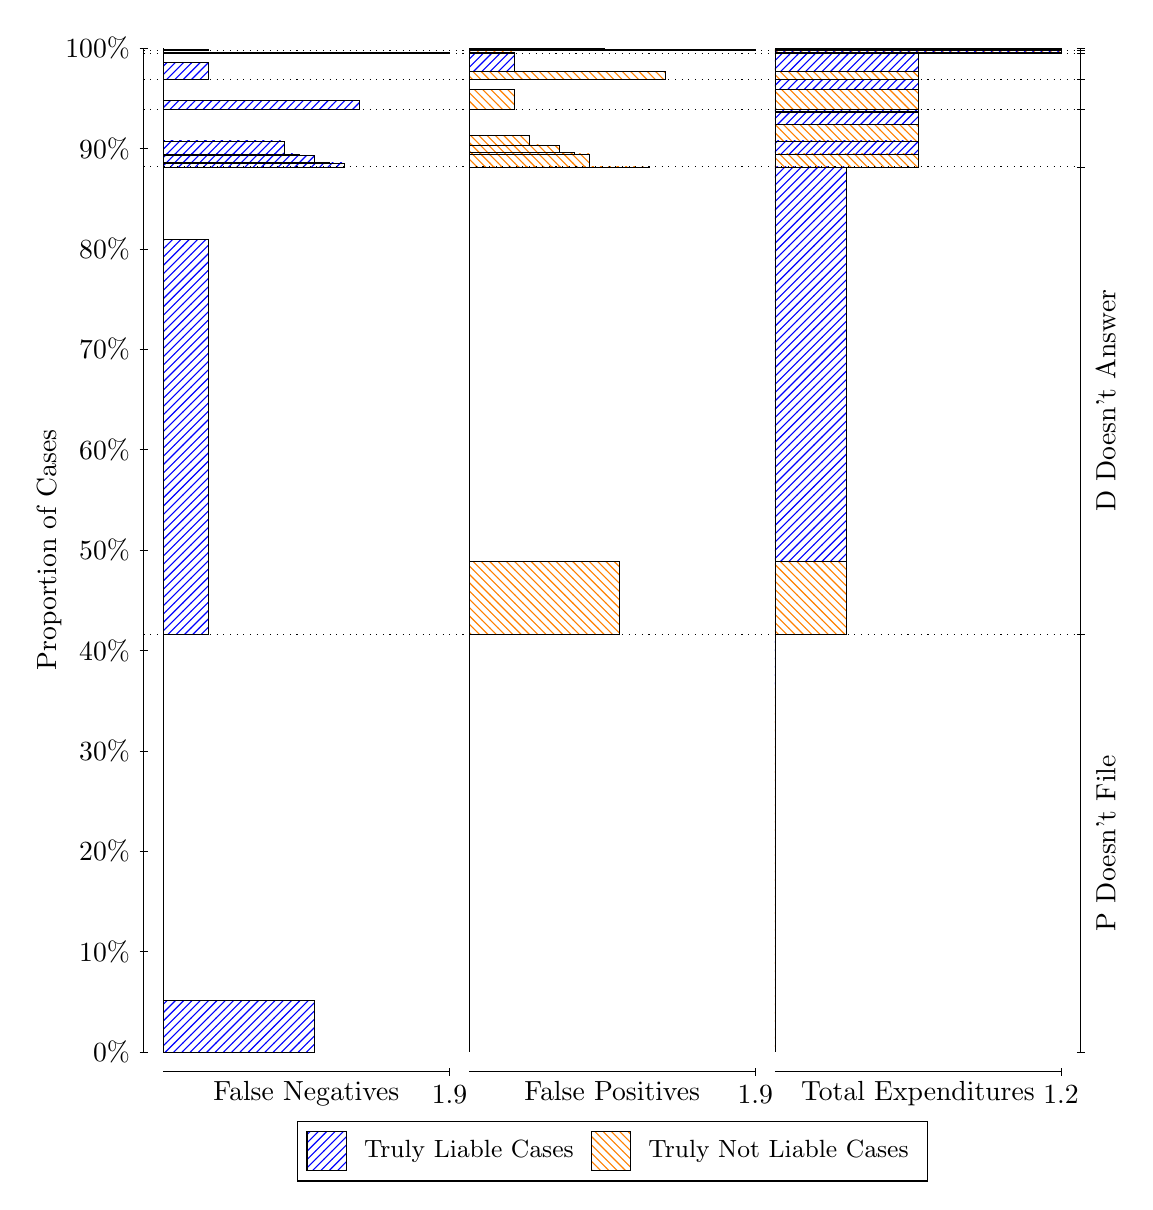
\begin{tikzpicture}
\draw[black, very thin] (1.5,1.75) -- (1.5,14.5);
\node[rotate=90, anchor=center] at (0.3, 8.125) {Proportion of Cases};
\draw[black, very thin] (1.45,1.75) -- (1.55,1.75);
\node[anchor=east] at (1.45, 1.75) {0\%};
\draw[black, very thin] (1.45,3.025) -- (1.55,3.025);
\node[anchor=east] at (1.45, 3.025) {10\%};
\draw[black, very thin] (1.45,4.3) -- (1.55,4.3);
\node[anchor=east] at (1.45, 4.3) {20\%};
\draw[black, very thin] (1.45,5.575) -- (1.55,5.575);
\node[anchor=east] at (1.45, 5.575) {30\%};
\draw[black, very thin] (1.45,6.85) -- (1.55,6.85);
\node[anchor=east] at (1.45, 6.85) {40\%};
\draw[black, very thin] (1.45,8.125) -- (1.55,8.125);
\node[anchor=east] at (1.45, 8.125) {50\%};
\draw[black, very thin] (1.45,9.4) -- (1.55,9.4);
\node[anchor=east] at (1.45, 9.4) {60\%};
\draw[black, very thin] (1.45,10.675) -- (1.55,10.675);
\node[anchor=east] at (1.45, 10.675) {70\%};
\draw[black, very thin] (1.45,11.95) -- (1.55,11.95);
\node[anchor=east] at (1.45, 11.95) {80\%};
\draw[black, very thin] (1.45,13.225) -- (1.55,13.225);
\node[anchor=east] at (1.45, 13.225) {90\%};
\draw[black, very thin] (1.45,14.5) -- (1.55,14.5);
\node[anchor=east] at (1.45, 14.5) {100\%};

\draw[black, very thin] (13.4,1.75) -- (13.4,14.5);
\draw[black, very thin] (13.35,1.75) -- (13.45,1.75);
\node[anchor=west] at (13.35, 1.75) {};
\draw[black, very thin] (13.35,7.0536) -- (13.45,7.0536);
\node[anchor=west] at (13.35, 7.0536) {};
\draw[black, very thin] (13.35,12.991) -- (13.45,12.991);
\node[anchor=west] at (13.35, 12.991) {};
\draw[black, very thin] (13.35,13.719) -- (13.45,13.719);
\node[anchor=west] at (13.35, 13.719) {};
\draw[black, very thin] (13.35,14.098) -- (13.45,14.098);
\node[anchor=west] at (13.35, 14.098) {};
\draw[black, very thin] (13.35,14.428) -- (13.45,14.428);
\node[anchor=west] at (13.35, 14.428) {};
\draw[black, very thin] (13.35,14.468) -- (13.45,14.468);
\node[anchor=west] at (13.35, 14.468) {};
\draw[black, very thin] (13.35,14.5) -- (13.45,14.5);
\node[anchor=west] at (13.35, 14.5) {};

\draw[black, very thin, pattern color=blue, pattern=north east lines] (1.75,1.75) rectangle (3.6623,2.4046);
\draw[black, very thin, pattern color=orange, pattern=north west lines] (1.75,2.4046) rectangle (1.75,7.0536);
\draw[black, very thin, pattern color=blue, pattern=north east lines] (1.75,7.0536) rectangle (2.3237,12.066);
\draw[black, very thin, pattern color=orange, pattern=north west lines] (1.75,12.066) rectangle (1.75,12.991);
\draw[black, very thin, pattern color=blue, pattern=north east lines] (1.75,12.991) rectangle (4.0447,13.042);
\draw[black, very thin, pattern color=blue, pattern=north east lines] (1.75,13.042) rectangle (3.8535,13.051);
\draw[black, very thin, pattern color=blue, pattern=north east lines] (1.75,13.051) rectangle (3.6623,13.137);
\draw[black, very thin, pattern color=blue, pattern=north east lines] (1.75,13.137) rectangle (3.4711,13.137);
\draw[black, very thin, pattern color=blue, pattern=north east lines] (1.75,13.137) rectangle (3.4711,13.157);
\draw[black, very thin, pattern color=blue, pattern=north east lines] (1.75,13.157) rectangle (3.2798,13.321);
\draw[black, very thin, pattern color=blue, pattern=north east lines] (1.75,13.321) rectangle (3.0886,13.322);
\draw[black, very thin, pattern color=blue, pattern=north east lines] (1.75,13.322) rectangle (2.8974,13.322);
\draw[black, very thin, pattern color=blue, pattern=north east lines] (1.75,13.322) rectangle (2.7061,13.322);
\draw[black, very thin, pattern color=blue, pattern=north east lines] (1.75,13.322) rectangle (2.5149,13.322);
\draw[black, very thin, pattern color=orange, pattern=north west lines] (1.75,13.322) rectangle (1.75,13.719);
\draw[black, very thin, pattern color=blue, pattern=north east lines] (1.75,13.719) rectangle (4.236,13.838);
\draw[black, very thin, pattern color=orange, pattern=north west lines] (1.75,13.838) rectangle (1.75,14.098);
\draw[black, very thin, pattern color=blue, pattern=north east lines] (1.75,14.098) rectangle (2.3237,14.322);
\draw[black, very thin, pattern color=orange, pattern=north west lines] (1.75,14.322) rectangle (1.75,14.428);
\draw[black, very thin, pattern color=blue, pattern=north east lines] (1.75,14.428) rectangle (5.3833,14.445);
\draw[black, very thin, pattern color=orange, pattern=north west lines] (1.75,14.445) rectangle (1.75,14.468);
\draw[black, very thin, pattern color=blue, pattern=north east lines] (1.75,14.468) rectangle (2.3237,14.485);
\draw[black, very thin, pattern color=orange, pattern=north west lines] (1.75,14.485) rectangle (1.75,14.5);
\draw[black, very thin, pattern color=orange, pattern=north west lines] (5.6333,1.75) rectangle (5.6333,6.3991);
\draw[black, very thin, pattern color=blue, pattern=north east lines] (5.6333,6.3991) rectangle (5.6333,7.0536);
\draw[black, very thin, pattern color=orange, pattern=north west lines] (5.6333,7.0536) rectangle (7.5456,7.9779);
\draw[black, very thin, pattern color=blue, pattern=north east lines] (5.6333,7.9779) rectangle (5.6333,12.991);
\draw[black, very thin, pattern color=orange, pattern=north west lines] (5.6333,12.991) rectangle (7.9281,12.991);
\draw[black, very thin, pattern color=orange, pattern=north west lines] (5.6333,12.991) rectangle (7.7368,12.991);
\draw[black, very thin, pattern color=orange, pattern=north west lines] (5.6333,12.991) rectangle (7.5456,12.991);
\draw[black, very thin, pattern color=orange, pattern=north west lines] (5.6333,12.991) rectangle (7.3544,12.991);
\draw[black, very thin, pattern color=orange, pattern=north west lines] (5.6333,12.991) rectangle (7.1632,13.156);
\draw[black, very thin, pattern color=orange, pattern=north west lines] (5.6333,13.156) rectangle (6.9719,13.175);
\draw[black, very thin, pattern color=orange, pattern=north west lines] (5.6333,13.175) rectangle (6.7807,13.261);
\draw[black, very thin, pattern color=orange, pattern=north west lines] (5.6333,13.261) rectangle (6.5895,13.271);
\draw[black, very thin, pattern color=orange, pattern=north west lines] (5.6333,13.271) rectangle (6.3982,13.388);
\draw[black, very thin, pattern color=blue, pattern=north east lines] (5.6333,13.388) rectangle (6.0158,13.388);
\draw[black, very thin, pattern color=blue, pattern=north east lines] (5.6333,13.388) rectangle (5.8246,13.388);
\draw[black, very thin, pattern color=blue, pattern=north east lines] (5.6333,13.388) rectangle (5.6333,13.719);
\draw[black, very thin, pattern color=orange, pattern=north west lines] (5.6333,13.719) rectangle (6.207,13.979);
\draw[black, very thin, pattern color=blue, pattern=north east lines] (5.6333,13.979) rectangle (5.6333,14.098);
\draw[black, very thin, pattern color=orange, pattern=north west lines] (5.6333,14.098) rectangle (8.1193,14.204);
\draw[black, very thin, pattern color=blue, pattern=north east lines] (5.6333,14.204) rectangle (6.207,14.428);
\draw[black, very thin, pattern color=orange, pattern=north west lines] (5.6333,14.428) rectangle (6.207,14.451);
\draw[black, very thin, pattern color=blue, pattern=north east lines] (5.6333,14.451) rectangle (5.6333,14.468);
\draw[black, very thin, pattern color=orange, pattern=north west lines] (5.6333,14.468) rectangle (9.2667,14.483);
\draw[black, very thin, pattern color=blue, pattern=north east lines] (5.6333,14.483) rectangle (7.3544,14.5);
\draw[black, very thin, pattern color=orange, pattern=north west lines] (9.5167,1.75) rectangle (9.5167,6.3991);
\draw[black, very thin, pattern color=blue, pattern=north east lines] (9.5167,6.3991) rectangle (9.5167,7.0536);
\draw[black, very thin, pattern color=orange, pattern=north west lines] (9.5167,7.0536) rectangle (10.425,7.9779);
\draw[black, very thin, pattern color=blue, pattern=north east lines] (9.5167,7.9779) rectangle (10.425,12.991);
\draw[black, very thin, pattern color=orange, pattern=north west lines] (9.5167,12.991) rectangle (11.333,13.155);
\draw[black, very thin, pattern color=blue, pattern=north east lines] (9.5167,13.155) rectangle (11.333,13.32);
\draw[black, very thin, pattern color=orange, pattern=north west lines] (9.5167,13.32) rectangle (11.333,13.533);
\draw[black, very thin, pattern color=blue, pattern=north east lines] (9.5167,13.533) rectangle (11.333,13.68);
\draw[black, very thin, pattern color=orange, pattern=north west lines] (9.5167,13.68) rectangle (11.333,13.699);
\draw[black, very thin, pattern color=blue, pattern=north east lines] (9.5167,13.699) rectangle (11.333,13.719);
\draw[black, very thin, pattern color=orange, pattern=north west lines] (9.5167,13.719) rectangle (11.333,13.979);
\draw[black, very thin, pattern color=blue, pattern=north east lines] (9.5167,13.979) rectangle (11.333,14.098);
\draw[black, very thin, pattern color=orange, pattern=north west lines] (9.5167,14.098) rectangle (11.333,14.204);
\draw[black, very thin, pattern color=blue, pattern=north east lines] (9.5167,14.204) rectangle (11.333,14.428);
\draw[black, very thin, pattern color=orange, pattern=north west lines] (9.5167,14.428) rectangle (13.15,14.451);
\draw[black, very thin, pattern color=blue, pattern=north east lines] (9.5167,14.451) rectangle (13.15,14.468);
\draw[black, very thin, pattern color=orange, pattern=north west lines] (9.5167,14.468) rectangle (13.15,14.483);
\draw[black, very thin, pattern color=blue, pattern=north east lines] (9.5167,14.483) rectangle (13.15,14.5);
\draw[black, dotted] (1.5,7.0536) -- (13.4,7.0536);
\draw[black, dotted] (1.5,12.991) -- (13.4,12.991);
\draw[black, dotted] (1.5,13.719) -- (13.4,13.719);
\draw[black, dotted] (1.5,14.098) -- (13.4,14.098);
\draw[black, dotted] (1.5,14.428) -- (13.4,14.428);
\draw[black, dotted] (1.5,14.468) -- (13.4,14.468);
\draw[black, very thin] (1.75,1.5) -- (5.3833,1.5);
\node[anchor=north] at (3.5667, 1.5) {False Negatives};
\draw[black, very thin] (5.3833,1.45) -- (5.3833,1.55);
\node[anchor=north] at (5.3833, 1.45) {1.9};

\draw[black, very thin] (5.6333,1.5) -- (9.2667,1.5);
\node[anchor=north] at (7.45, 1.5) {False Positives};
\draw[black, very thin] (9.2667,1.45) -- (9.2667,1.55);
\node[anchor=north] at (9.2667, 1.45) {1.9};

\draw[black, very thin] (9.5167,1.5) -- (13.15,1.5);
\node[anchor=north] at (11.333, 1.5) {Total Expenditures};
\draw[black, very thin] (13.15,1.45) -- (13.15,1.55);
\node[anchor=north] at (13.15, 1.45) {1.2};

\node[black, centered, rotate=90] at (13.72, 4.4018) {P Doesn't File};
\node[black, centered, rotate=90] at (13.72, 10.022) {D Doesn't Answer};






\draw (7.449999999999999,1.5) node[draw=none] (baseCoordinate) {};
\begin{scope}[align=center]
        \matrix[scale=0.5, draw=black, below=0.5cm of baseCoordinate, nodes={draw}, column sep=0.1cm]{
            \node[rectangle, draw, minimum width=0.5cm, minimum height=0.5cm, pattern=north east lines, pattern color=blue] {}; &
            \node[draw=none, font=\small] (B) {Truly Liable Cases}; &
            \node[rectangle, draw, minimum width=0.5cm, minimum height=0.5cm, pattern=north west lines, pattern color=orange] {}; &
            \node[draw=none, font=\small] (B) {Truly Not Liable Cases}; \\
            };
\end{scope}

\end{tikzpicture}
\end{document}